\chapter{Tutorial}
\label{chpt:Tutorial}
\typeout{$Id$}

\section{What you should put in .xsession or .xinitrc}

The scripts .xsession (called from xdm, gdm, etc.) or .xinitrc (called
from xinit or startx) control what happens when you log in or start X. 
Typically this file initializes your X11 environment.  To use
TkSessionManager, you should have 

\begin{verbatim}
path/to/TkSessionManager
\end{verbatim}

as the last (eg after things like calls to xrdb or xset or xmodmap) or
only thing in this file.  TkSessionManager will launch your window
manager (eg fvwm) and run a script that starts your default
applications. 

\section{Initial Configuration}

TkSessionManager reads in the file \$HOME/.tksessionmanagerrc using
Tcl/Tk \texttt{option readfile} command.  This file is formatted like a
standard X11 resource file\footnote{Much like .XResources or
.Xdefaults.} and generally contains resource settings used by
TkSessionManager.  The main resources used are:

\begin{description}
\item[*MenuFilename] This is the path of the menu file to use to build
the command menu.
\item[*MainTitle] This is the main title text to use.
\item[*MainGeometry] This is the geometry to use for the main
TkSessionManager window.
\item[*PrintCommand] This is the command to print the contents of the
text area.
\item[*WindowManager] This is the path to the window manager to launch.
\item[*SessionScript] This is the path of the session start up script to
use.
\item[*GnomeSettingsDaemon] This is a flag to indicate whether or not to
start the Gnome Settings Daemon.
\item[*GnomeScreensaver] This is a flag to indicate whether or not to
allow the Gnome Screensaver (started by the Gnome Settings Daemon) to run.
\end{description}

\begin{figure}[hbpt]
\begin{centering}
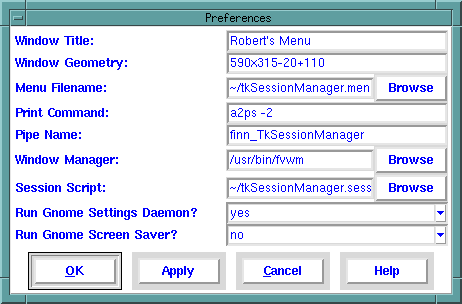
\includegraphics[width=5in]{PreferencesEditor.png}
\caption{Preferences Editor Window.}
\label{tut:fig:preferenceseditor}
\end{centering}
\end{figure}
You might want to initially create this file with a text editor
\textit{before} starting TkSessionManager for the first time.  This will
insure that there are sensible values.  Although TkSessionManager has
default values for all of the options and will start without this file
being present, the defaults might not always be sensible, depending on
you particular system setup.  All of these options can also be edited
with the TkSessionManager itself by selecting the \texttt{Preferences}
menu item on the \texttt{Edit} menu, as shown in
Figure~\ref{tut:fig:preferenceseditor}. The Preferences Editor Window is
described in detail in Section~\ref{sect:EditPreferences}.

You will very much want to create the session start up script yourself,
although it too is optional.  You will also want to make sure you have a
configuration file for your window manager as well!

\section{Creating a Launcher Menu}

\begin{figure}[hbpt]
\begin{centering}
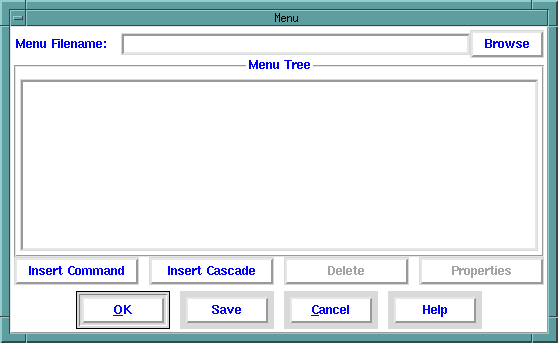
\includegraphics[width=5in]{MenuEditor.png}
\caption{Menu Editor Window.}
\label{tut:fig:menueditor}
\end{centering}
\end{figure}
You can either create a Launcher Menu using a text editor or you can use
the Menu Editor, as shown in Figure~\ref{tut:fig:menueditor}.  The Menu
Editor is started from the \texttt{Menu} menu item on the \texttt{Edit}
menu. The Menu Editor is described in detail in
Section~\ref{sect:EditCommandMenu}. 



\section{Using the text area}


The text area is just a plain text area which accepts keyboard input
with basic Emacs-like bindings.  It can be pasted to from the X11 copy
buffer and the text in it can be selected and copied to the X11 copy
buffer.  The contents of this text area can be saved to a text file
(\texttt{Save As} menu item on the \texttt{Session} menu) or sent to
the printer (\texttt{Print} menu item on the \texttt{Session} menu). 
The text area can be completely cleared with the \texttt{Clear} menu
item on the \texttt{Session} menu.  In addition, anything written to the
named pipe gets appended to the end of the text area, so it is possible
to capture the stdout and/or stderr streams from processes (all
processes launched from the \texttt{Commands} menu have their stdout and
stderr streams directed to this pipe).

